\chapter{Исследовательский раздел}

Предметом исследований является скорость и пропускная способность сервера при запросе картинки. Нагрузочное тестирование проводилось на примере изображения в формате PNG размером 2.8 Мбайт. Сравнивались разработанный сервер и Nginx~\cite{dejonghe2020nginx}.

Характеристики устройства, на котором проводилось исследование, следующие~\cite{macbook}:

\begin{itemize}
 \item оперативная память 16Гб;
 \item процессор Apple M2 Air;
 \item операционная система macOS Ventura 13.0.1.
\end{itemize}

Оба сервера были запущены в Docker~\cite{docker} со следующими ограничениями по ресурсам: оперативная память~---~2Гб, ресурс процессора~---~2000m.

Зависимости количества запросов, обрабатываемых серверов в секунду, от количества потоков представлена на рисунке \ref{img:plot}.

\begin{figure}[h!]
    \centering
    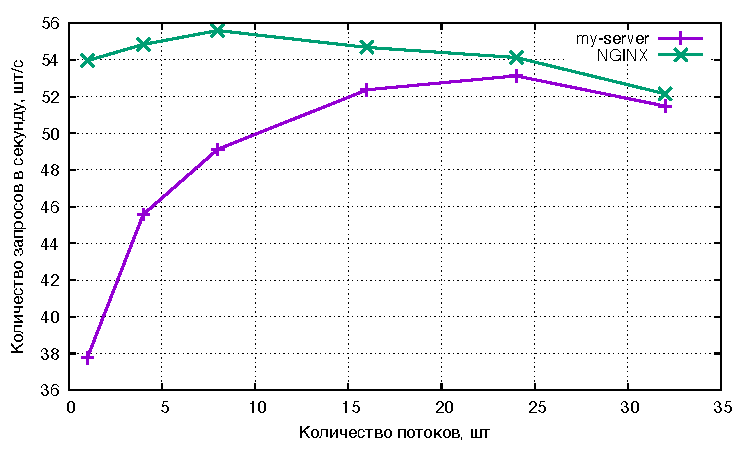
\includegraphics[scale=0.8]{assets/plot.pdf}
    \caption{Зависимости ... от количества потоков}
    \label{img:plot}
\end{figure}

По графику видно, что NGINX обрабатывает большее количество запросов в секунду, чем разработанный сервер. При 1 потоке он быстрее в 1.43 раз, при 32 потоках в 1.01 раз.